\chapter {Fase I: Análisis}
\label{cap:Fase I. Análisis}

Hasta hace algo más de una década, las recomendaciones clínicas en la prevención cardiovascular iban dirigidas fundamentalmente al manejo independiente de sus factores de riesgo. Con este enfoque, y de forma sistemática, se fueron elaborando guías para el abordaje de cada uno de los factores de riesgo. Sin embargo,  nuestro trabajo se apoya en estudios que toman los factores de riesgo como un conjunto para realizar una estimación precisa de la probabilidad de sufrir una enfermedad cardiovascular. 


\section{Factores de Riesgo cardiovascular}
Los factores de riesgo cardiovascular son condicionantes ligados a estilos de vida que incrementan la probabilidad de padecer o morir por enfermedad vascular en aquellas personas en las que inciden. Se catalogan como tales cuando cumplen unos requisitos que permiten establecer una relación de causa-efecto con respecto a la enfermedad vascular. Se pueden clasificar como se muestra en la siguiente figura. Subrayados en amarillo se muestran los que utiliza el algoritmo de Framimgham, tal y como se explicará más adelante. 

\begin{figure}[htb]
	\centering
	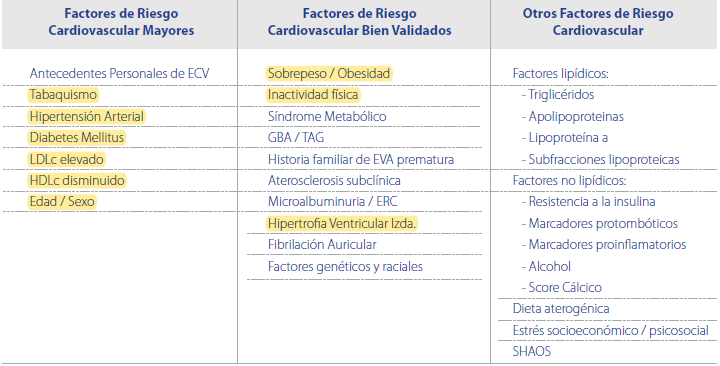
\includegraphics[width=\textwidth]{factores} 
	\caption[Tabla Factores]{Factores de Riesgo Cardiovascular (FRCV) \cite{tagle2007estimacion}
	}
	\label{fig:factores}
\end{figure}

Estos factores de riesgo cardiovasculares, ya sea de forma aislada o como sucede con mucha mayor frecuencia, en combinación, explican la mayoría de casos de enfermedad vascular o de muerte que ocurre en individuos de alto riesgo y una proporción considerable de casos en la población general.


\section{Estimación del Riesgo cardiovascular}
El Riesgo Cardiovascular expresa la probabilidad de sufrir un evento de la enfermedad vascular en un determinado período de tiempo, generalmente 5 o 10 años. La explicación en la práctica de este hecho es que de 100 personas con un mismo porcentaje de riesgo cardiovascular (Ej. RCV de 21\%), de esas 100 personas, 21 desarrollaran una Enfermedad Vascular en los próximos 5 o 10 años.

Para la prevención cardiovascular es necesaria una valoración conjunta de los factores de riesgo mediante la estimación del riesgo cardiovascular del individuo. Esto, permite definir niveles de riesgo con los que el personal sanitario y los propios pacientes pueden valorar cómo se modifica el mismo a medida que se van logrando los objetivos pactados.

Existen diversos métodos para estimar el RCV y ninguno de ellos es perfecto. Sin embargo, se ha comprobado que son las\textbf{ tablas de
Framingham } las que mejor se comportan a la hora de predecir la aparición de eventos cardiovasculares:

\begin{itemize}
\item Tienen \textbf{riesgo cardiovascular alto} los pacientes que reúnen una puntuación de Framingham de 22 o superior, lo que supone una probabilidad de padecer un evento cardiovascular en los próximos 10 años superior al 20\%. También consideraremos en riesgo alto a aquellos que ya han sufrido un episodio cardiovascular o presentan diabetes. 

\item Se califican de \textbf{riesgo cardiovascular moderado} aquellos pacientes con factor de riesgo (hipertensión arterial o tabaquismo) y una puntuación inferior al 22, y consiguientemente una probabilidad de episodio isquémico inferior al 20\% en los próximos 10 años.

\item Son de \textbf{riesgo cardiovascular bajo} los pacientes, independientemente de la edad y el sexo, sin factores de riesgos reconocidos. 
\end{itemize}

El cálculo de valoración al que nos referimos se reproduce en las tablas ~\ref{fig:raCalculo1} y ~\ref{fig:raCalculo2}. Es importante tener en cuenta que existen factores de riesgo cardiovascular no incluidos en la tabla, como el sedentarismo, obesidad, y sobre todo el antecedente familiar aparecido en edad precoz (antes de 55 años en familiares varones y de 65 en mujeres), que deben ser considerados para establecer un plan personalizado de control de riesgo en cada paciente.  
\begin{figure}[htb]
	\centering
	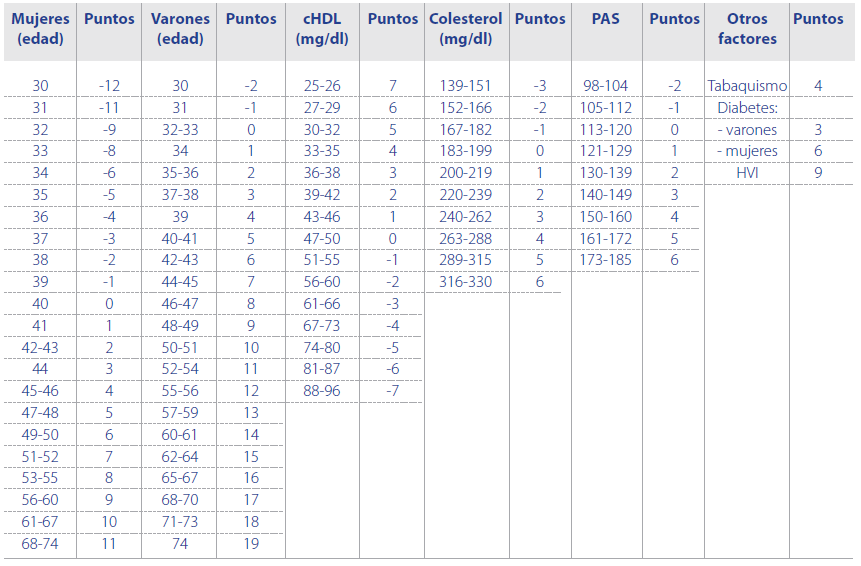
\includegraphics[width=\textwidth]{tablaFir} 
	\caption[Tabla Framighan]{Tablas de cálculos de RCV del estidoo de Framingham (Anderson, 1991) \cite{tagle2007estimacion}
	}
	\label{fig:tablaFir1}
\end{figure}

\begin{figure}[htb]
	\centering
	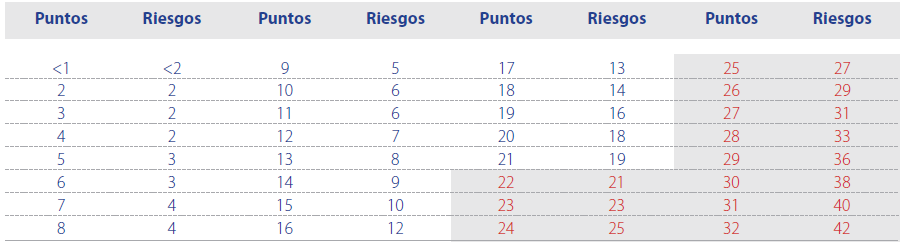
\includegraphics[width=\textwidth]{tablaFir2} 
	\caption[Predicción Framighan]{Tabla de puntuación y porcentaje de riesgo en los próximos 10 años \cite{tagle2007estimacion}
	}
	\label{fig:tablaFir2}
\end{figure}





\section{Implementando el Algoritmo de Framingham}
Una vez estudiado qué es y cómo se estima el riesgo cardiovascular, el objetivo que nos proponemos en este trabajo es el desarrollo de una aplicación que implemente el algoritmo de Framimgham, de forma que, para la información particular introducida por un sujeto, sea capaz de calcular el porcentaje de riesgo de sufrir una enfermedad cardiovascular en un periodo de 10 años. 

La utilidad práctica del uso de la tabla, y consecuentemente de nuestra aplicación, radica en que permite:
\begin{itemize}
\item Priorizar los cuidados, controles y seguimientos en aquellas personas que presentan un mayor riesgo.

\item Apoyar en las decisiones de tratamiento farmacológico en cuanto a hipolipemiantes, antihipertensivos y antiagregantes.

\item Monitorizar la evolución del RCV

\item Constituir una herramienta educativa y motivacional para el paciente en cuanto a la obtención de objetivos para la reducción de su riesgo.
\end{itemize}



